\newcommand{\env}[1]{\texttt{#1}}
\newcommand{\command}[1]{\texttt{#1}}
\newcommand{\package}[1]{\texttt{\itshape#1}}
\newcommand{\engl}[1]{(engl: \textit{#1})\xspace}
\setlength{\parindent}{0pt}
\lstset{extendedchars=\true}
\lstset{inputencoding=ansinew}
\newcommand\tab[1][1cm]{\hspace*{#1}}
\newpage

\section{Aufgabe 1 - Firewall mit IPTables}

\subsection{Teilaufgabe a)}

\subsubsection{Frage- bzw. Aufgabenstellung}

Welche Ports verwenden die Programme zur Kommunikation? Wie ändert man die Standardeinstellungen? Ist dazu ein Neustart des Systems nötig?

\subsubsection{Lösung}

Bei Linux Betriebssystemen kann man sich  die verwendeten Ports mit dem Befehl \textit{netstat -tulpn} anzeigen lassen. netstat ist ein häufig benutztes Diagnose-Werkzeug um verschiedene Informationen über die Netzwerkschnittstellen anzeigen zu lassen. Die Portnummer sieht man dann in der Spalte \textit{Local Address} nach dem letzten Doppelpunkt. Dies sollte dann so aussehen: 

\begin{figure}[htbp]
\begin{center}
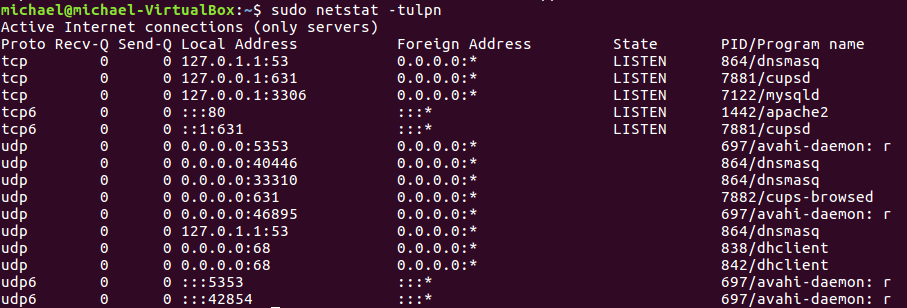
\includegraphics[width=0.7\textwidth]{Bild1}
\caption{Portnummer anzeigen lassen}
\end{center}
\end{figure}

\subsubsection{Ergebnis}

Wir können die verschiedenen Ports der Programme auslesen.

\subsection{Teilaufgabe b)} \cite{1,2}

\subsubsection{Frage- bzw. Aufgabenstellung}

Richten Sie eine restriktive Firewall ein (prohibitive Sicherheitspolitik). Es soll sichergestellt werden, dass ausschließlich der Port des Webservers von außen zugänglich ist. Die Firewall soll automatisch beim Start des Systems geladen werden. Nutzen Sie für die Lösung der Aufgabe ausschließlich die Kommandozeile und das Kommando iptables. 

\subsubsection{Lösung}

Da der Webserver den Port 80 (localhost) besitzt, müssen wir dafür sorgen, dass nur eingehende Pakete für diesen Port angenommen werden und sonst keine. Dafür benutzen wir den Befehl \textit{iptables -A INPUT -i lo -j ACCEPT}. Das -A hängt eine Regel an die \textit{Chain} an, dass -i ist für die Netzwerkschnittstelle zuständig über die Pakete eingehen (in diesem Fall localhost) und das -j legt die Aktion fest. Anschließend benutzen wir noch den Befehl \textit{iptables -A INPUT -j DROP} damit keine weiteren Pakete angenommen werden. Daher auch der Command \textit{DROP}. Diese Befehle schreiben wir in eine neue Datei im init.d Ordner über den Command \\
\textit{touch /etc/init.d/firewall \&\& chmod 755 /etc/init.d/firewall \&\& nano /etc/init.d/firewall}. \\ Damit das Skript bei jedem Neustart ausgeführt wird, schreiben wir folgenden Code in die \textit{rc.local}-Datei:

\begin{lstlisting}[caption={rc.local}]
if [ -e '/etc/init.d/firewall' ]
then
    /bin/sh '/etc/init.d/firewall'
fi
\end{lstlisting}

\subsubsection{Ergebnis}

Wir können mit \textit{iptables} eine Firewall einstellen und sorgen dafür, dass die Firewall bei jedem Systemstart aktiv ist.

\subsection{Teilaufgabe d)} \cite{3}

\subsubsection{Frage- bzw. Aufgabenstellung}

Nun öffnen Sie mit netcat auf dem Rechner A (eine Ihrer VMs) ein oder zwei Ports zwischen 0 und 100. Nutzen Sie dafür den Befehl: nc -l [Portnummer].\\
\\
nmap ist ein Portscanner, mit dem man u.a. die eigene Firewall auf Sicherheitslücken testen kann. Mit \\
nmap Zieladresse -p [Anfangsport]-[Endport] \\
kann nach offenen Ports in einem bestimmten Portbereich gescannt werden. Führen Sie nun einen Portscan auf VM A von VM B aus. Welches Ergebnis sehen Sie?

\subsubsection{Lösung}

Zunächst öffnen wir den Port 48 mit dem Befehl \textit{nc -l 48}. Anschließend scannen wir den Port mit dem Befehl \textit{nmap localhost -p 48}. Wie man in Abbildung ~\ref{fig:Portscan} erkennen kann, bekommt man die Ausgabe dass der Port offen ist (STATE -> open). Wenn ich nun von einer anderen VM einen Portscan ausführe, wird auch hier erkannt dass der Port mit der Nummer 48 auf der VM A offen ist (siehe Abbildung ~\ref{fig:Portscan2}). 

\begin{figure}[htbp]
\begin{center}
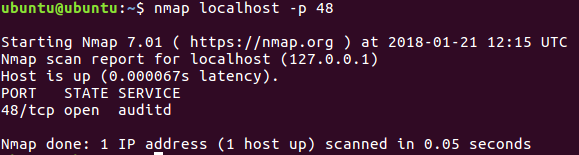
\includegraphics[width=0.7\textwidth]{Bild2}
\caption{Portscan mit nmap}
\label{fig:Portscan}
\end{center}
\end{figure}

\begin{figure}[htbp]
\begin{center}
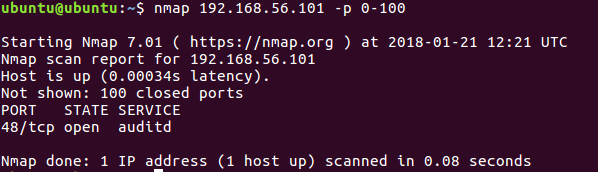
\includegraphics[width=0.7\textwidth]{Bild3}
\caption{Portscan von anderer VM}
\label{fig:Portscan2}
\end{center}
\end{figure}

\newpage

\subsubsection{Ergebnis}

Wir können mit dem Befehl netcat verschiedene Ports öffnen und nmap anwenden um einen Portscan durchzuführen.

\subsection{Teilaufgabe e)} \cite{4}

\subsubsection{Frage- bzw. Aufgabenstellung}

Definieren Sie nun Regeln mit iptables, die einen solchen Scan blocken. Dazu bietet es sich an, alle Pakete zu verwerfen, die ungewöhnlich schnell Verbindungsanfragen senden. \\
Sehen Sie sich die folgende Regel an und versuchen Sie zu verstehen, welchen Sinn einzelne Befehle erfüllen. Sie werden sie im Verlauf dieser Übung noch benötigen. Wenden Sie diese Regel an. Die zweite Regel soll nun bei genau solchen Paketen in der gleichen Liste nachsehen, ob die Adresse eines Paketes bereits eingetragen ist. Trifft dies zu, soll die letzte Zeitmarke upgedatet werden. Wenn nun ein und dieselbe Adresse versucht 20 oder mehr Verbindungsanfragen innerhalb von 10 Sekunden zu senden, sollen all diese Pakete verworfen werden. Wie sieht die entsprechenede Regel aus? Testen Sie die Funktionalität der Regeln mit nmap.

\subsubsection{Lösung}

Die Regel \textit{iptables -A INPUT -p tcp -i eth1 -m state --state NEW -m recent --set} sagt zunächst am Anfang, dass es sich um eine Regel handelt die eine neue Chain vom Typ INPUT anhängt (-A INPUT). Des weiteren wird mit dem Befehl \textit{-p} gesagt, dass nur Pakete vom Protokoll tcp überprüft werden und die \textit{-i} Option sagt aus, dass nur Pakete von der Netzwerkschnittstelle \textit{eth1} überprüft werden. Weiterhin wird noch gesagt, dass nur Pakete mit dem Status \textit{NEW} überprüft werden. \textit{recent} erlaubt es dynamisch Listen mit IP-Adressen zu erstellen und dann an Hand der Listen Pakete zu filtern. Die zweite Regel würde dann so aussehen:

\begin{lstlisting}[caption={iptables mit "recent"}]
iptables -A INPUT -p tcp -i eth1 -m state --state ESTABLISHED -m recent --update --seconds 10 --hitcount 20 -j REJECT --reject-with tcp-reset
\end{lstlisting}

Mit dem Befehl \textit{--update} fügen wir einen weiteren Zeitstempel ein, welcher dann mit \textit{--seconds} überprüft ob in den letzten 10 Sekunden 20 weitere Zeitstempel vorliegen (\textit{--hitcount}). Wenn das der Fall ist, wird die Verbindung zurückgesetzt (\textit{-j REJECT --reject-with tcp-reset}.


\subsubsection{Ergebnis}

Wir können Regeln mit iptables aufstellen, die dafür sorgen, dass gewisse Scans blockiert werden.

\subsection{Teilaufgabe f)} \cite{5}

\subsubsection{Frage- bzw. Aufgabenstellung}

Nun sollen die Portscans mithilfe der LOG-Funktion protokolliert werden. Dazu kann zuerst eine neue Kette für Portscans mit Namen PORTSCAN o.ä. erstellt werden. Als zweites muss eine Regel definiert werden, die alle Pakete in dieser Kette protokolliert. Als Log-Prefix soll "PORTSCAN erkannt --" verwendet werden. iptables loggt i.d.R. in der Datei /var/log/syslog. Kontrollieren Sie, ob Ihre Ausgabe in der Logdatei erscheint.

\subsubsection{Lösung}

Zunächst erstellen wir eine neue Kette mit dem Namen PORTSCAN (siehe Zeile 1). Anschließend definieren wir eine Regel damit alle Pakete dieser Kette protokolliert werden (siehe Zeile 2).

\begin{lstlisting}[caption={Portscan protokollieren}]
sudo iptables -N PORTSCAN
sudo iptables -A PORTSCAN -j LOG --log-prefix "PORTSCAN erkannt --"
\end{lstlisting}

Danach erstellen wir eine einfache Regel fest, die die eingehende Kommunikation für localhost zulässt. Als Aktion nehmen wir diesmal aber \textit{PORTSCAN} (siehe Zeile 1).

\begin{lstlisting}[caption={Regel für PORTSCAN}]
sudo iptables -A INPUT -i lo -j PORTSCAN
\end{lstlisting}

Wenn jetzt mit nmap ein Portscan durchgeführt wird, kann man in der \textit{syslog}-Datei sehen, dass unsere Ausgabe dort erscheint (Abbildung ~\ref{fig:syslog}).

\begin{figure}[htbp]
\begin{center}
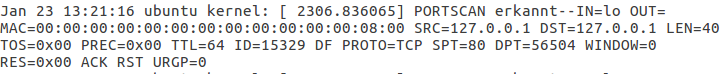
\includegraphics[width=0.7\textwidth]{Bild4}
\caption{Ausgabe in syslog}
\label{fig:syslog}
\end{center}
\end{figure}

\subsubsection{Ergebnis}

Wir können unsere Portscans mit der LOG-Funktion protokollieren.

\subsection{Teilaufgabe g)}

\subsubsection{Frage- bzw. Aufgabenstellung}

Hping3 ist ein Tool, um die eigene Firewall zu testen. Es kann benutzerdefinierte TCP-Pakete generieren und das auch mit langsamerer Geschwindigkeit als nmap. Schicken Sie einer VM mehrere TCP-Pakete mit gesetzter SYN-Flag beginnend mit Port 0. \\
\\
Welchen Befehl verwenden Sie und woran erkennt man, welche Ports offen sind?

\subsubsection{Lösung}

Wir konnten diese Aufgabe nicht bearbeiten, da wir das Paket hping3 nicht installieren konnten.



\section{Quellen}
\begin{thebibliography}{999}
\bibitem {1} damadmai, iptables2 \\ \url{https://wiki.ubuntuusers.de/iptables2/}, 23.01.2018 
\bibitem {2} Markus Mansshardt, iptables Firewall-Script für Debian \\ \url{http://blog.mansshardt.net/iptables-firewall-script-fuer-debian/}, 23.01.2018
\bibitem {3} Heinrich Schwietering, netcat \\ \url{https://wiki.ubuntuusers.de/netcat/}, 23.01.2018
\bibitem {4} heise.de, SSH vor Brute-Force-Angriffen schützen \\ \url{https://www.heise.de/security/artikel/recent-271032.html}, 23.01.2018
\bibitem {5} FK, Portscans mit iptables erkennen und protokollieren. \\ \url{https://www.kworx.de/portscans-iptables-protokollieren/}, 23.01.2018

\end{thebibliography}




